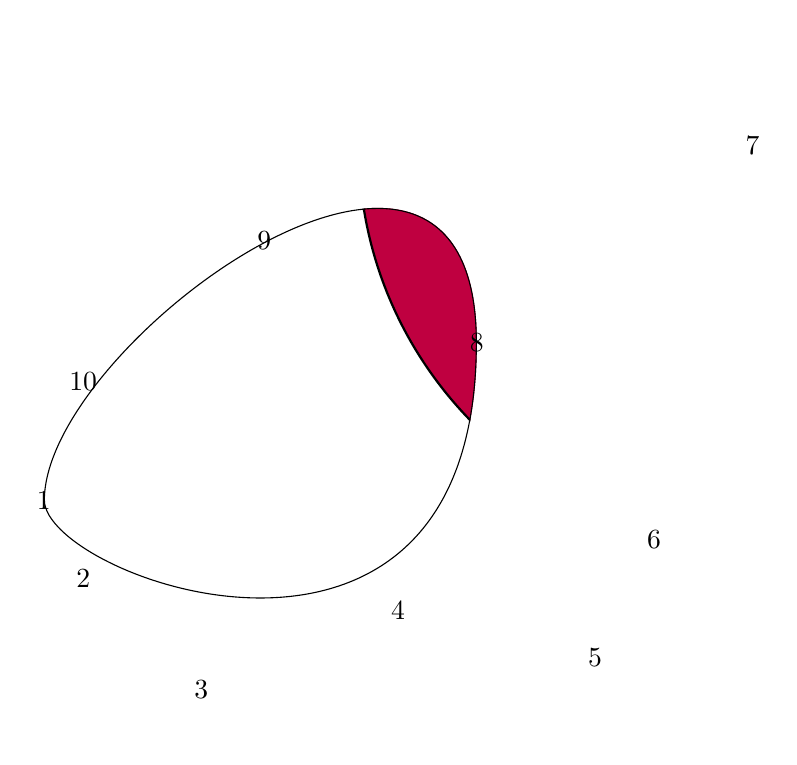
\begin{tikzpicture}
	%\draw[help lines] (0,0) grid (15,10);

	\path
	coordinate (aux0) at (0,1.5)
	coordinate (aux1) at (0,3.5)
	coordinate (aux2) at (10,3.5)
	coordinate (aux3) at (9,6)
	coordinate (aux4) at (4,0)
	coordinate (aux5) at (7,0)
	coordinate (aux6) at (2,6)
	coordinate (aux7) at (5,6)
	coordinate (esp1) at (1,2.5)
	coordinate (esp2) at (1.5,1.5)
	coordinate (esp3) at (3,0.1)
	coordinate (esp4) at (5.5,1.1)
	coordinate (esp5) at (8,0.5)
	coordinate (esp6) at (8.75,2)
	coordinate (esp7) at (10,7)
	coordinate (esp8) at (6.5,4.5)
	coordinate (esp9) at (3.8,5.8)
	coordinate (esp10) at (1.5,4)
	;



	% \def\regionA{(esp1) to [out=-90,in=-180]
	%  % (esp2) to [out=-10,in=170]
	%   (esp3) to [out=0, in=-120]
	%   (esp4) to [out=60,in=-90]
	% %   (esp5) to[out=10,in=-150]
	% %  % (esp6) to[out=20,in=-90]
	% %   (esp7) to[out=90,in=-180]
	%    (esp8) to[out=90,in=0]
	%    (esp9) to[out=-180,in=90]
	%  %  (esp10) to[out=180,in=90]
	%   cycle;  }

	\def\regionA{

		(esp1) .. controls +(0,2) and + (0,4) .. (esp8)
		.. controls +(0,-5) and + (0,-1) ..
		cycle;
	}

	\def\regionB{(esp7) circle (5cm);}


	% \draw%[fill=gray!30] 
	%     (esp1) .. controls +(0,4) and + (0,4) .. (esp8)
	%           .. controls +(0,-5) and + (0,-1) .. 
	%           cycle;

	\begin{scope}
		\clip
		\regionA
		\fill[fill=purple]
		\regionB
		\draw[line width=0.8pt]\regionB
		\draw[line width=0.8pt]\regionA
	\end{scope}

	% \filldraw[fill=cyan!40]
	%   (aux4) to[bend right=10]
	%   (aux6) --
	%   (aux7) to[bend left=10]
	%   (aux5) -- cycle;
	% \filldraw[fill=brown!60]
	%   (aux5) to[bend right=10]
	%   (aux7) --
	%   (10,6) --
	%   (10,0) -- cycle;
	% \filldraw[fill=green!30]
	%   (aux0) -- 
	%   (aux1) to[bend right=10]
	%   (aux3) --
	%   (10,6) -- 
	%   (aux2) to[bend left=10] cycle;
	% \filldraw[fill=yellow!50]
	%   (0,0) -- 
	%   (aux4) to[bend right=10]
	%   (aux6) --
	%   (0,6) -- 
	%   (0,0) -- cycle;
	% \filldraw[fill=orange!40]
	%   (0,6) -- 
	%   (aux1) to[bend right=10]
	%   (aux3) --
	%   (0,6) -- cycle;
	% \node at (4,5) {$E_1$};  
	% \node at (2,2) {$E_2$};  
	% \node at (6,3.3) {$E_3$};  
	% \node at (4.4,1.3) {$E_4$};  
	% \node at (7.5,2) {$E_5$};  

	\node at (esp1) {1};
	\node at (esp2) {2};
	\node at (esp3) {3};
	\node at (esp4) {4};
	\node at (esp5) {5};
	\node at (esp6) {6};
	\node at (esp7) {7};
	\node at (esp8) {8};
	\node at (esp9) {9};
	\node at (esp10) {10};

\end{tikzpicture}